% Compact single-column motivation, introduced at its first reference.
\begin{figure}[t]
  \centering
  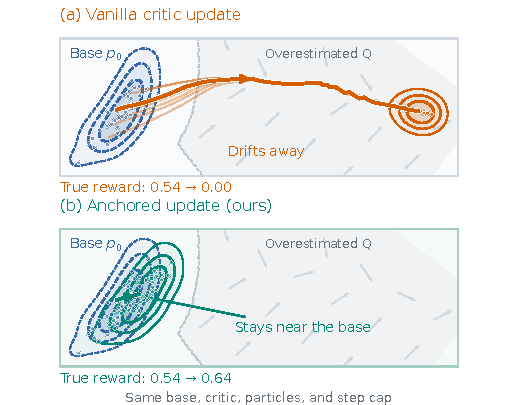
\includegraphics[width=\linewidth]{figures/problem_motivation.pdf}
  \caption{\textbf{Distribution drift under a misleading critic.}
  Blue shows an analytic base policy; orange and green show $384$ paired
  particles after $60$ critic-ascent updates without and with anchoring.
  Contours enclose $50/80/95\%$ of the estimated probability mass; dots and
  paths show representative particles. Gray arrows follow increasing critic
  value in an overestimated region. Scores are particle averages.
  This single-seed toy uses $25$ critic-training samples and a $0.06$ step
  cap. Projection within $0.15$ of each particle's base action illustrates
  CAST's anchoring principle, rather than full policy training.}
  \label{fig:problem}
\end{figure}
